\documentclass[12pt,a4paper]{article}
\usepackage[utf8x]{inputenc}
\usepackage{ucs}
\usepackage[english,russian]{babel}
\usepackage[OT1]{fontenc}
\usepackage{amsmath}
\usepackage{amsfonts}
\usepackage{amssymb}
\usepackage{wasysym}
\usepackage{physics}
\usepackage{wrapfig}
\usepackage{mathrsfs}

%\usepackage{graphicx}
%\usepackage{float}
%\usepackage{tikz}
%\usepackage{misccorr}
%\usepackage{booktabs}
%\usepackage{siunitx}

%---------Схемы---------
\usepackage{circuitikz}
%-----------------------

%--------Графики--------
\usepackage{pgfplots}
%Чтобы хорошо работало
\pgfplotsset{compat=1.9}
%----------------------

\usepackage[left=2cm,right=2cm,top=2cm,bottom=2cm,includefoot,footskip=1.5cm]{geometry}

\usepackage{fancyhdr}
\pagestyle{fancy}

\usepackage[T1]{fontenc}
 
\usepackage{indentfirst}
%% Sets page size and margins
%\usepackage[dvips]{graphicx}
%\graphicspath{{noiseimages/}}
%\usepackage[colorinlistoftodos]{todonotes}
%\usepackage[colorlinks=true, allcolors=blue]{hyperref}

\rhead{\small Д.\,Павлов, МФТИ}
\lhead{Лабораторная работа №3.6.1}

\author{Дмитрий Павлов, 790}
\title {\textbf{Спектральный анализ электрических сигналов.}}

\begin{document}
\maketitle
\newpage
\tableofcontents 

\newpage

\section{Вступление.}
    \subsection{Цель работы.}
        Изучение спектрального состава периодических электрических сигналов.
        
    \subsection{Оборудование.}
        \begin{itemize}
            \item Персональный компьютер;
            \item USB-осциллограф АКИП-4107;
            \item Функциональный генератор WaveStation 2012;
            \item Соединительные кабели.
        \end{itemize}

    \subsection{Экспериментальная установка.}
        Функциональный генератор WaveStation 2012 позволяет сформировать два различных электрических сигнала, которые выводятся на два независимых канала - <<CH1>> и <<CH2>>. Сигнал с каналов подается на входы осциллографа. Затем эти сигналы подаются на вход компьютера через USB-соединение. В режиме спектроанализатора можно наблюдать спектры этих сигналов.

\section{Словарь.}
    1. Спектр сигнала - разложение сигнала на более простые в базисе ортогональных функций.
    
    2. Амплитудная модуляция - вид модуляции, при которой изменяемым параметром несущего сигнала является его амплитуда.
    
    3. Пусть заданная $f(t)$ периодически повторяется с частотой $\Omega_1 = 2\pi/T$, $T$ -- период повторения.
    Ее разложение в ряд Фурье:
    \[
    f(t) = \dfrac{a_0}{2} + \sum_{n=1}^{\infty} [a_n \cos{n\Omega_1 t} + b_n, \sin{n\Omega_2 t}]
    \]
    \[
    a_n = \dfrac{2}{T}\int_{t_1}^{t_1 + T} f(t) \cos{n\Omega_1 t}dt,
    \]
    \[
    b_n = \dfrac{2}{T}\int_{t_1}^{t_1 + T} f(t) \sin{n\Omega_1 t}dt.
    \]
    Амплитуда и фаза $n$-й гармоники:
    \[
    A_n = \sqrt{a_n^2 + b_n^2},
    \]
    \[
    \psi_n = \arctan{\dfrac{b_n}{a_n}}.
    \]
\newpage

\section{Практическая часть.}
    \subsection{Исследуем спектр периодической последовательности прямоугольных импульсов.}
        
        Проанализируем, как меняется спектр при увеличении длительности импульсов или частоте повтора вдвое.
        \begin{center}
            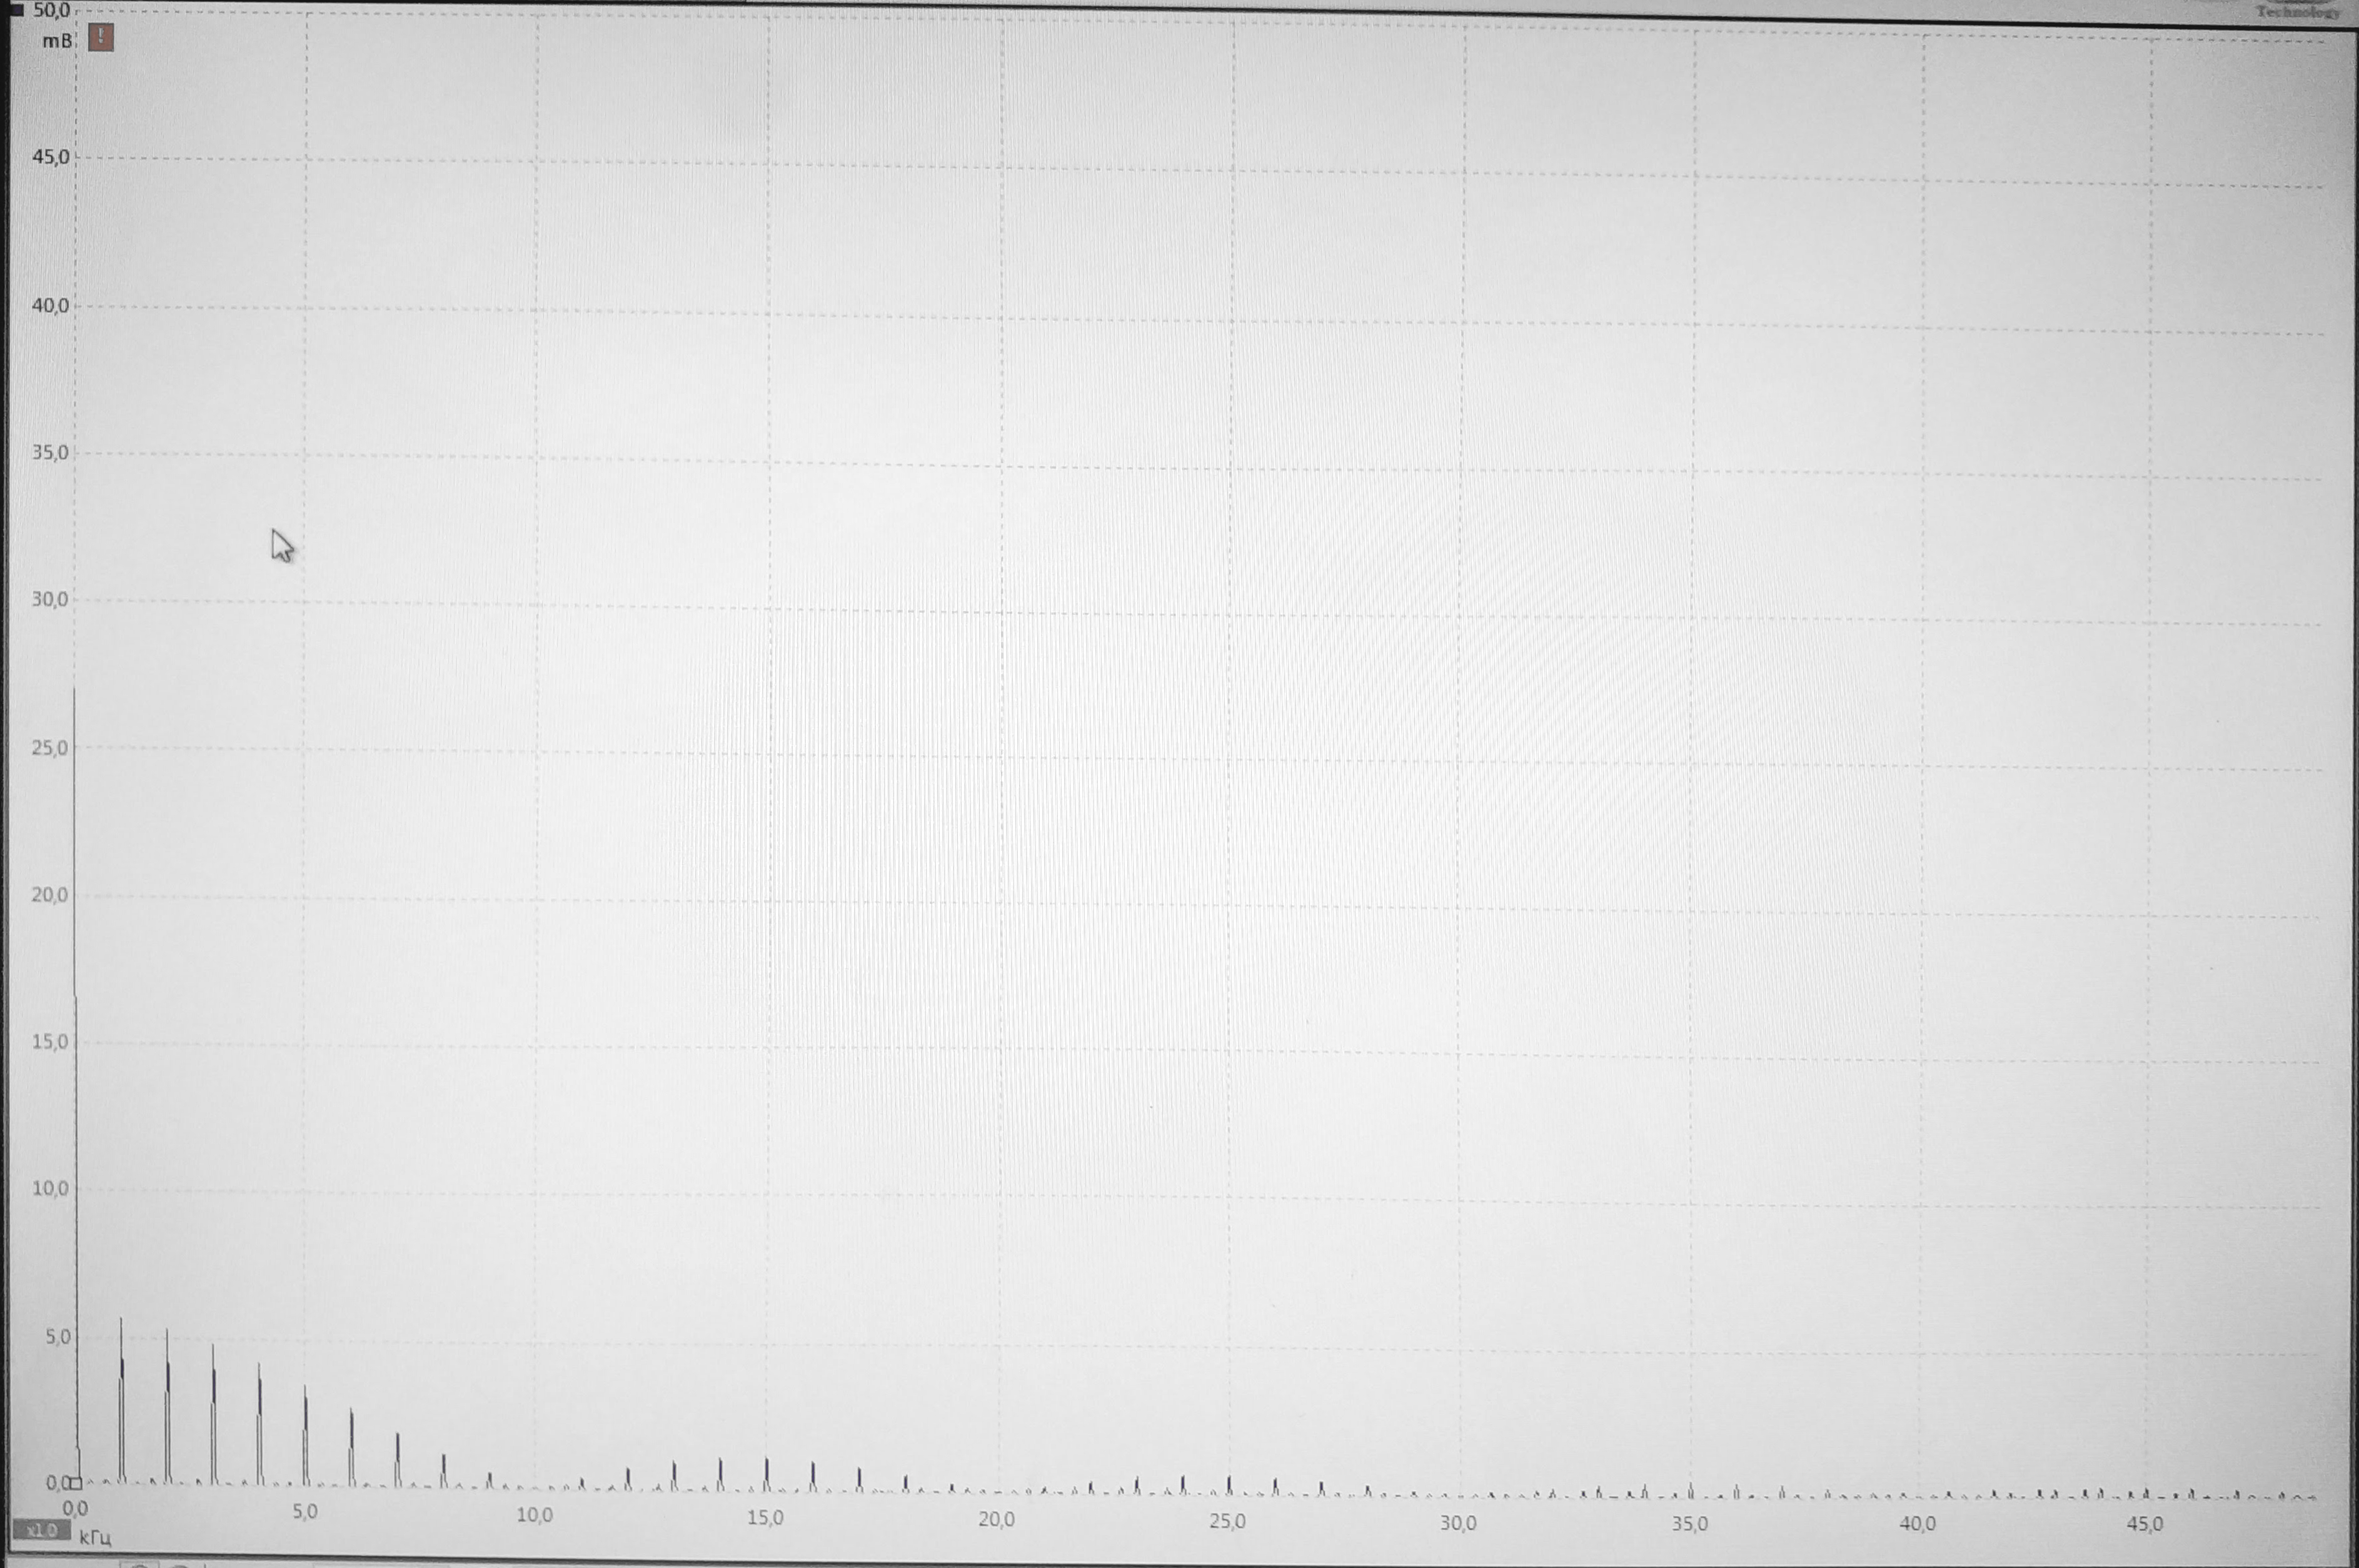
\includegraphics[width=0.85\linewidth]{img/9.jpg}
       
            При $\tau = 100 \si{\micro\second}$, $f_{\text{повт}} = 1\si{\kilo\hertz}$. 
            \includegraphics[width=0.85\linewidth]{img/10.jpg}
            
            При увеличении $\tau$ вдвое.
        
            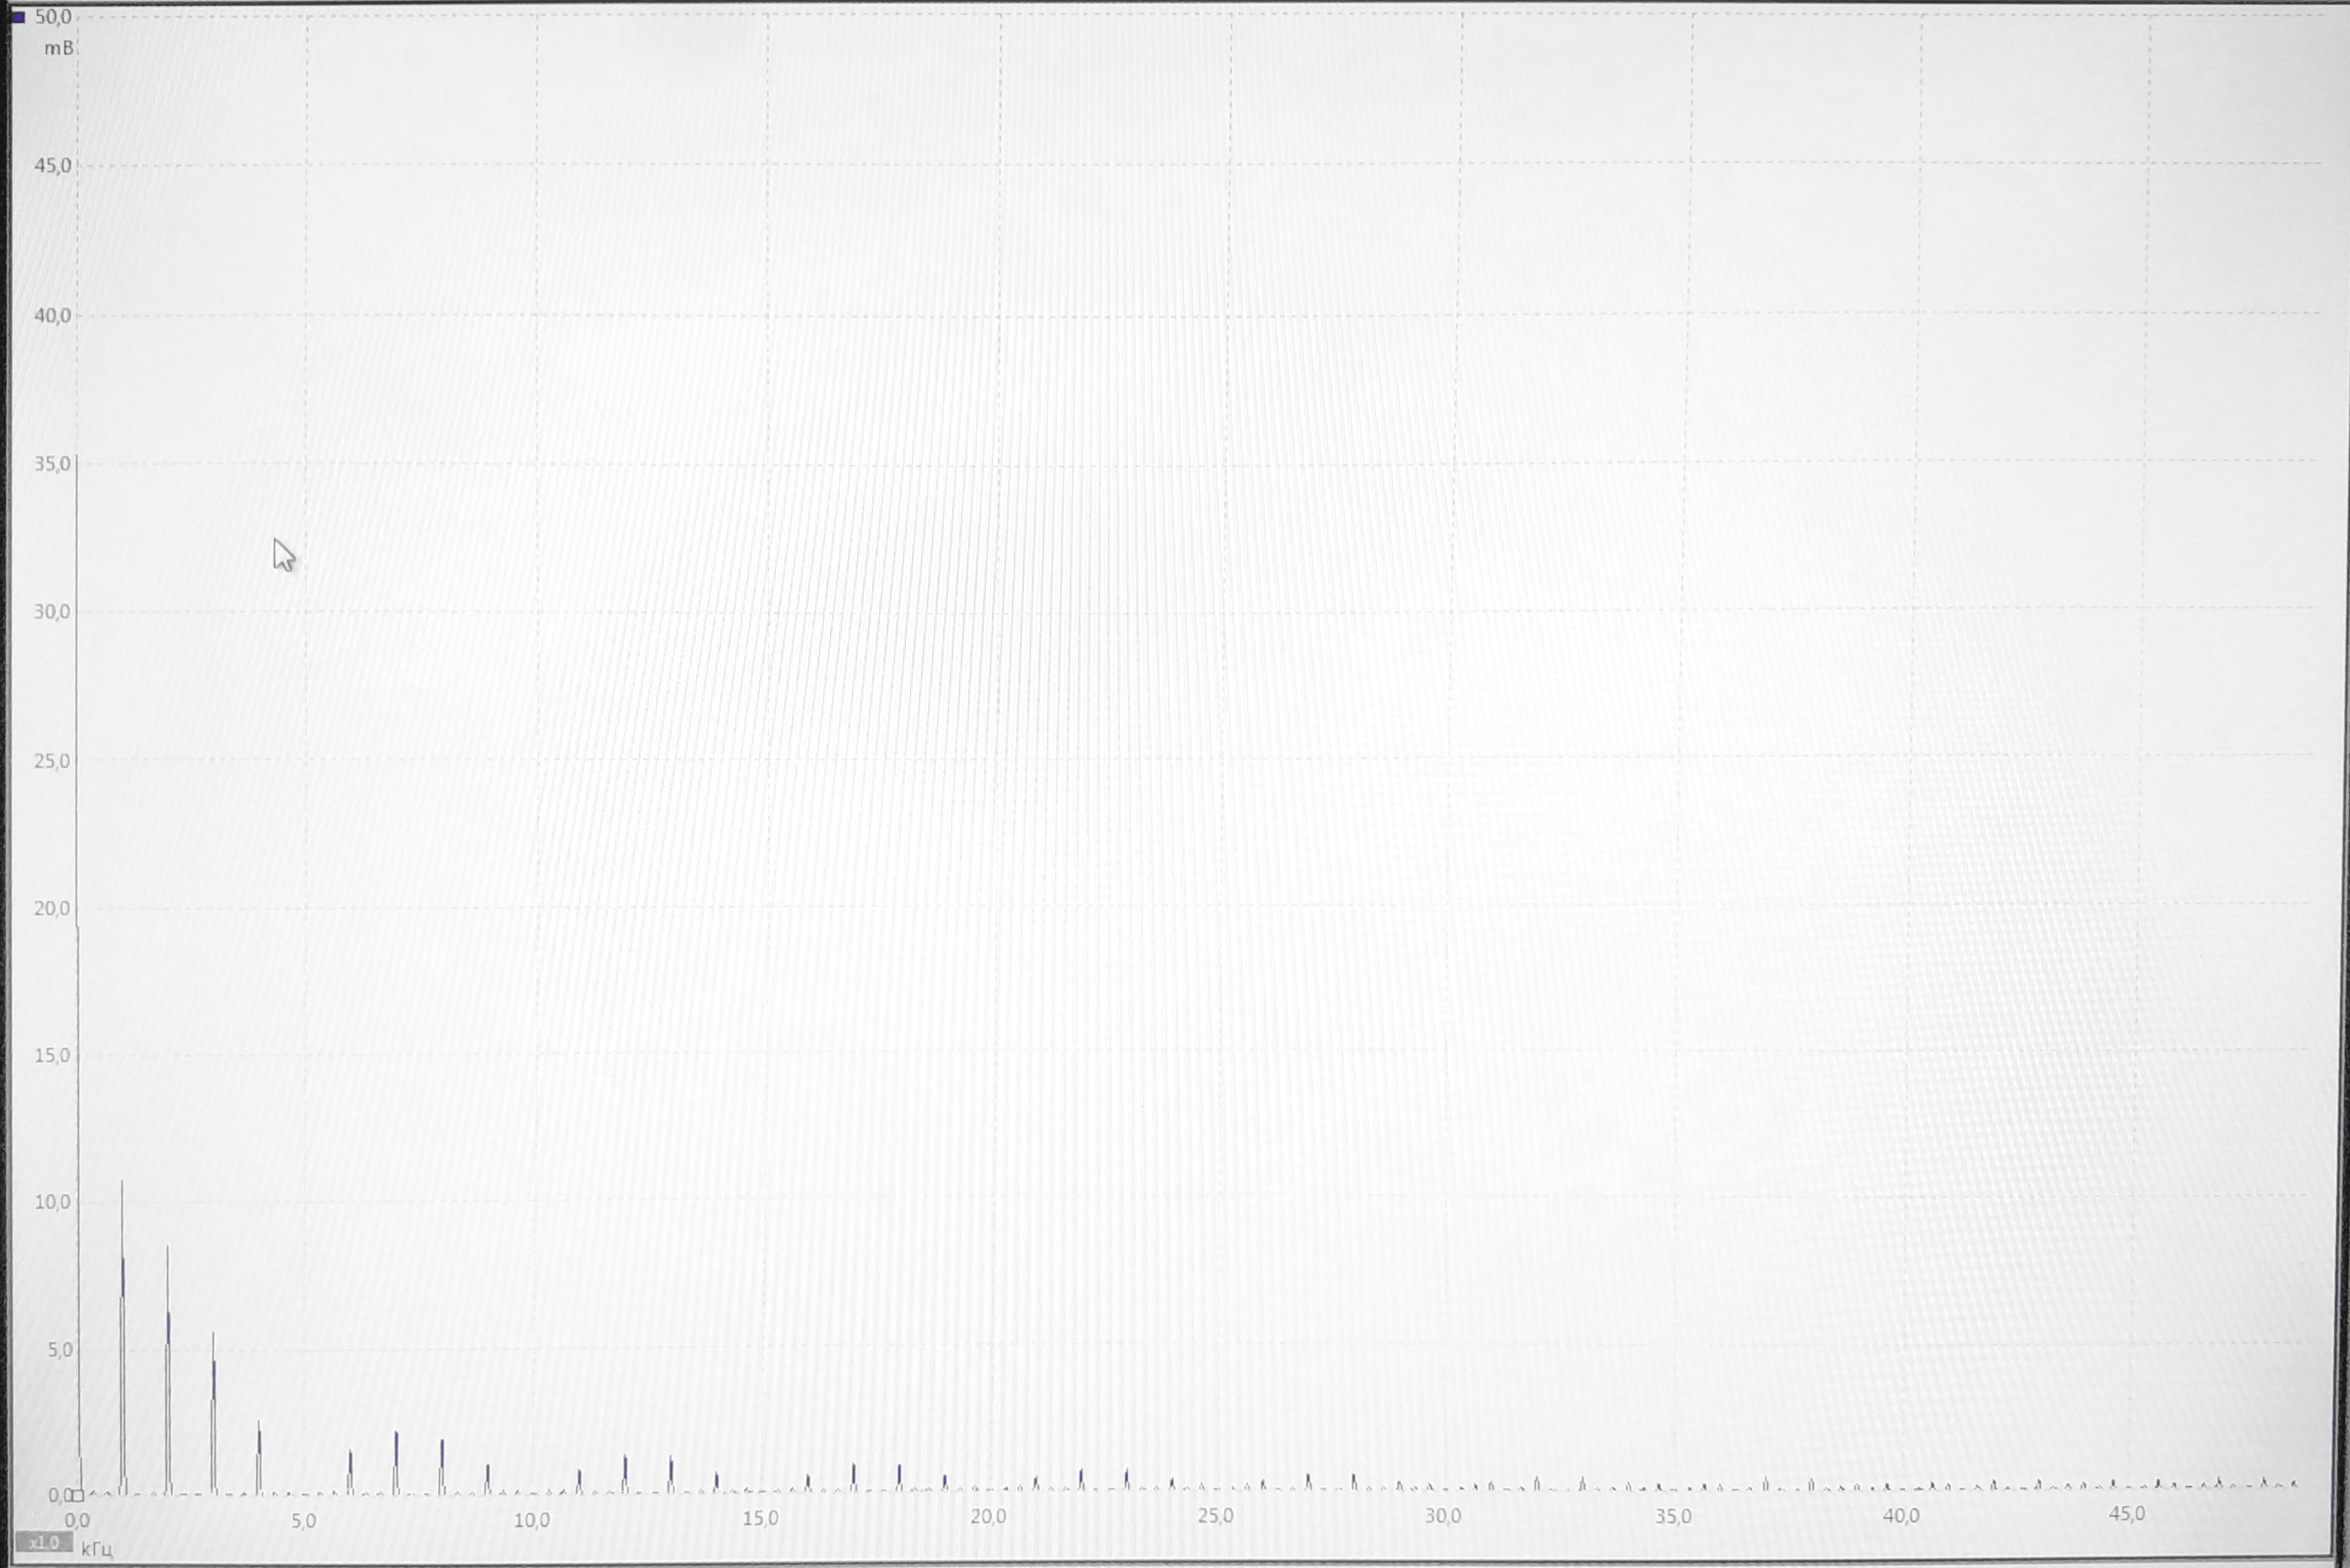
\includegraphics[width=0.85\linewidth]{img/8.jpg}
        
            При увеличении $f_{\text{повт}}$ вдвое.
        \end{center}
        
        \newpage
        Проведем измерения зависимости ширины спектра $\Delta \upsilon$ от длительности импульса $\tau$:
        
        \begin{center}
            \begin{tabular}{|c|r|r|r|r|r|r|r|r|r|r|}
            \hline
                 N  &   1   &   2   &   3   &   4   &   5   &   6   &   7   &   8   &   9   &   10                      \\ \hline
                 $\Delta \upsilon, \si{\kilo\hertz}$ & 25.0 & 17.0 & 13.0 & 11.0 & 9.0 & 8.0 & 7.0 & 6.0 & 5.5 & 5.0    \\ \hline
                 $\tau, \si{\micro\second}$ & 40.0 & 57.8 & 75.6 & 93.3 & 111.1 & 128.9 & 146.7 & 164.4 & 182.2 & 200.0 \\ \hline
            \end{tabular}
        \end{center}

        Построим график.
        \begin{center}
            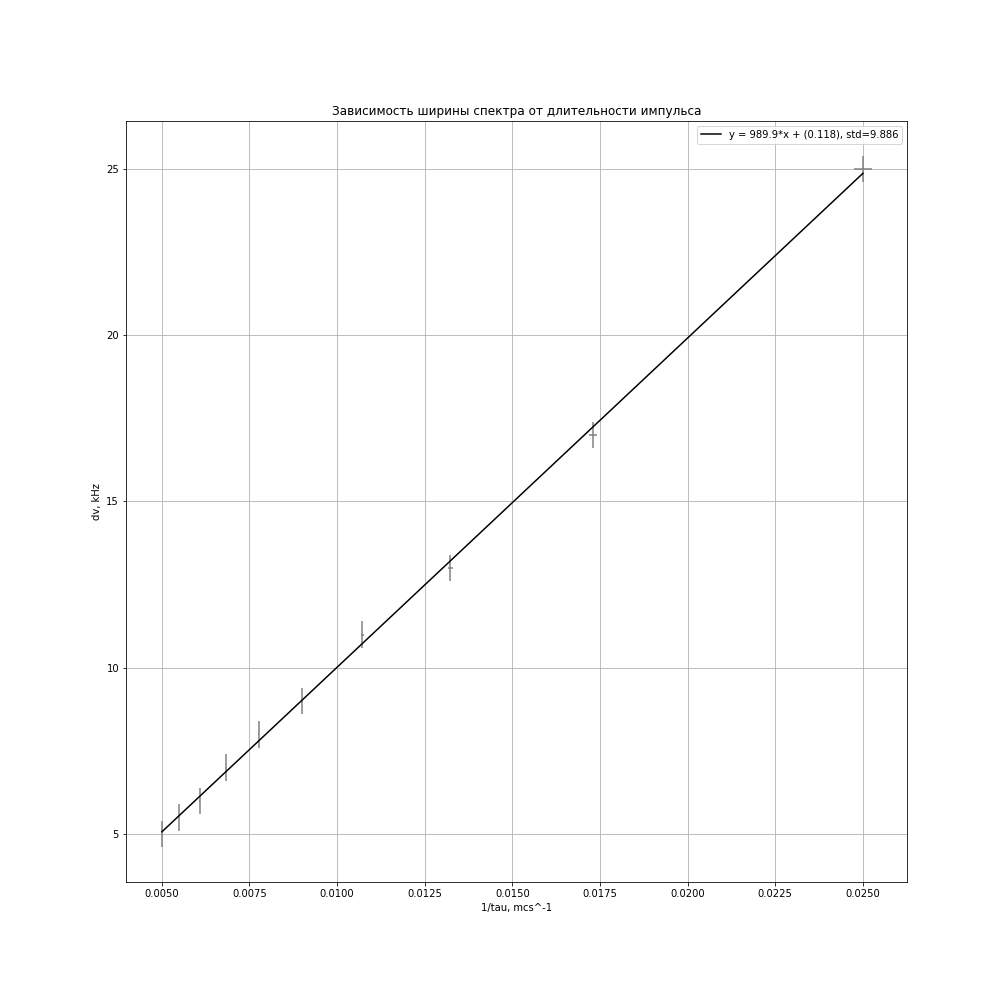
\includegraphics[width=\linewidth]{img/1.png}
        \end{center}
        
        Видим, что по наклону прямой можно убедиться в справедливости соотношения неопределенностей.
    
    \subsection{Исследуем спектр периодической последовательности цугов гармонических колебаний.}
        Установим длительность импульса $\tau = 100 \si{\micro\second}$. Проследим, как меняется картина спектра при изменении несущей частоты.
        \begin{center}
            \includegraphics[width=0.9\linewidth]{img/11.jpg}

            При $\upsilon_0 = 25 \si{\kilo\hertz}$.
        
            \includegraphics[width=0.85\linewidth]{img/12.jpg}

            При $\upsilon_0 = 10 \si{\kilo\hertz}$.
        
            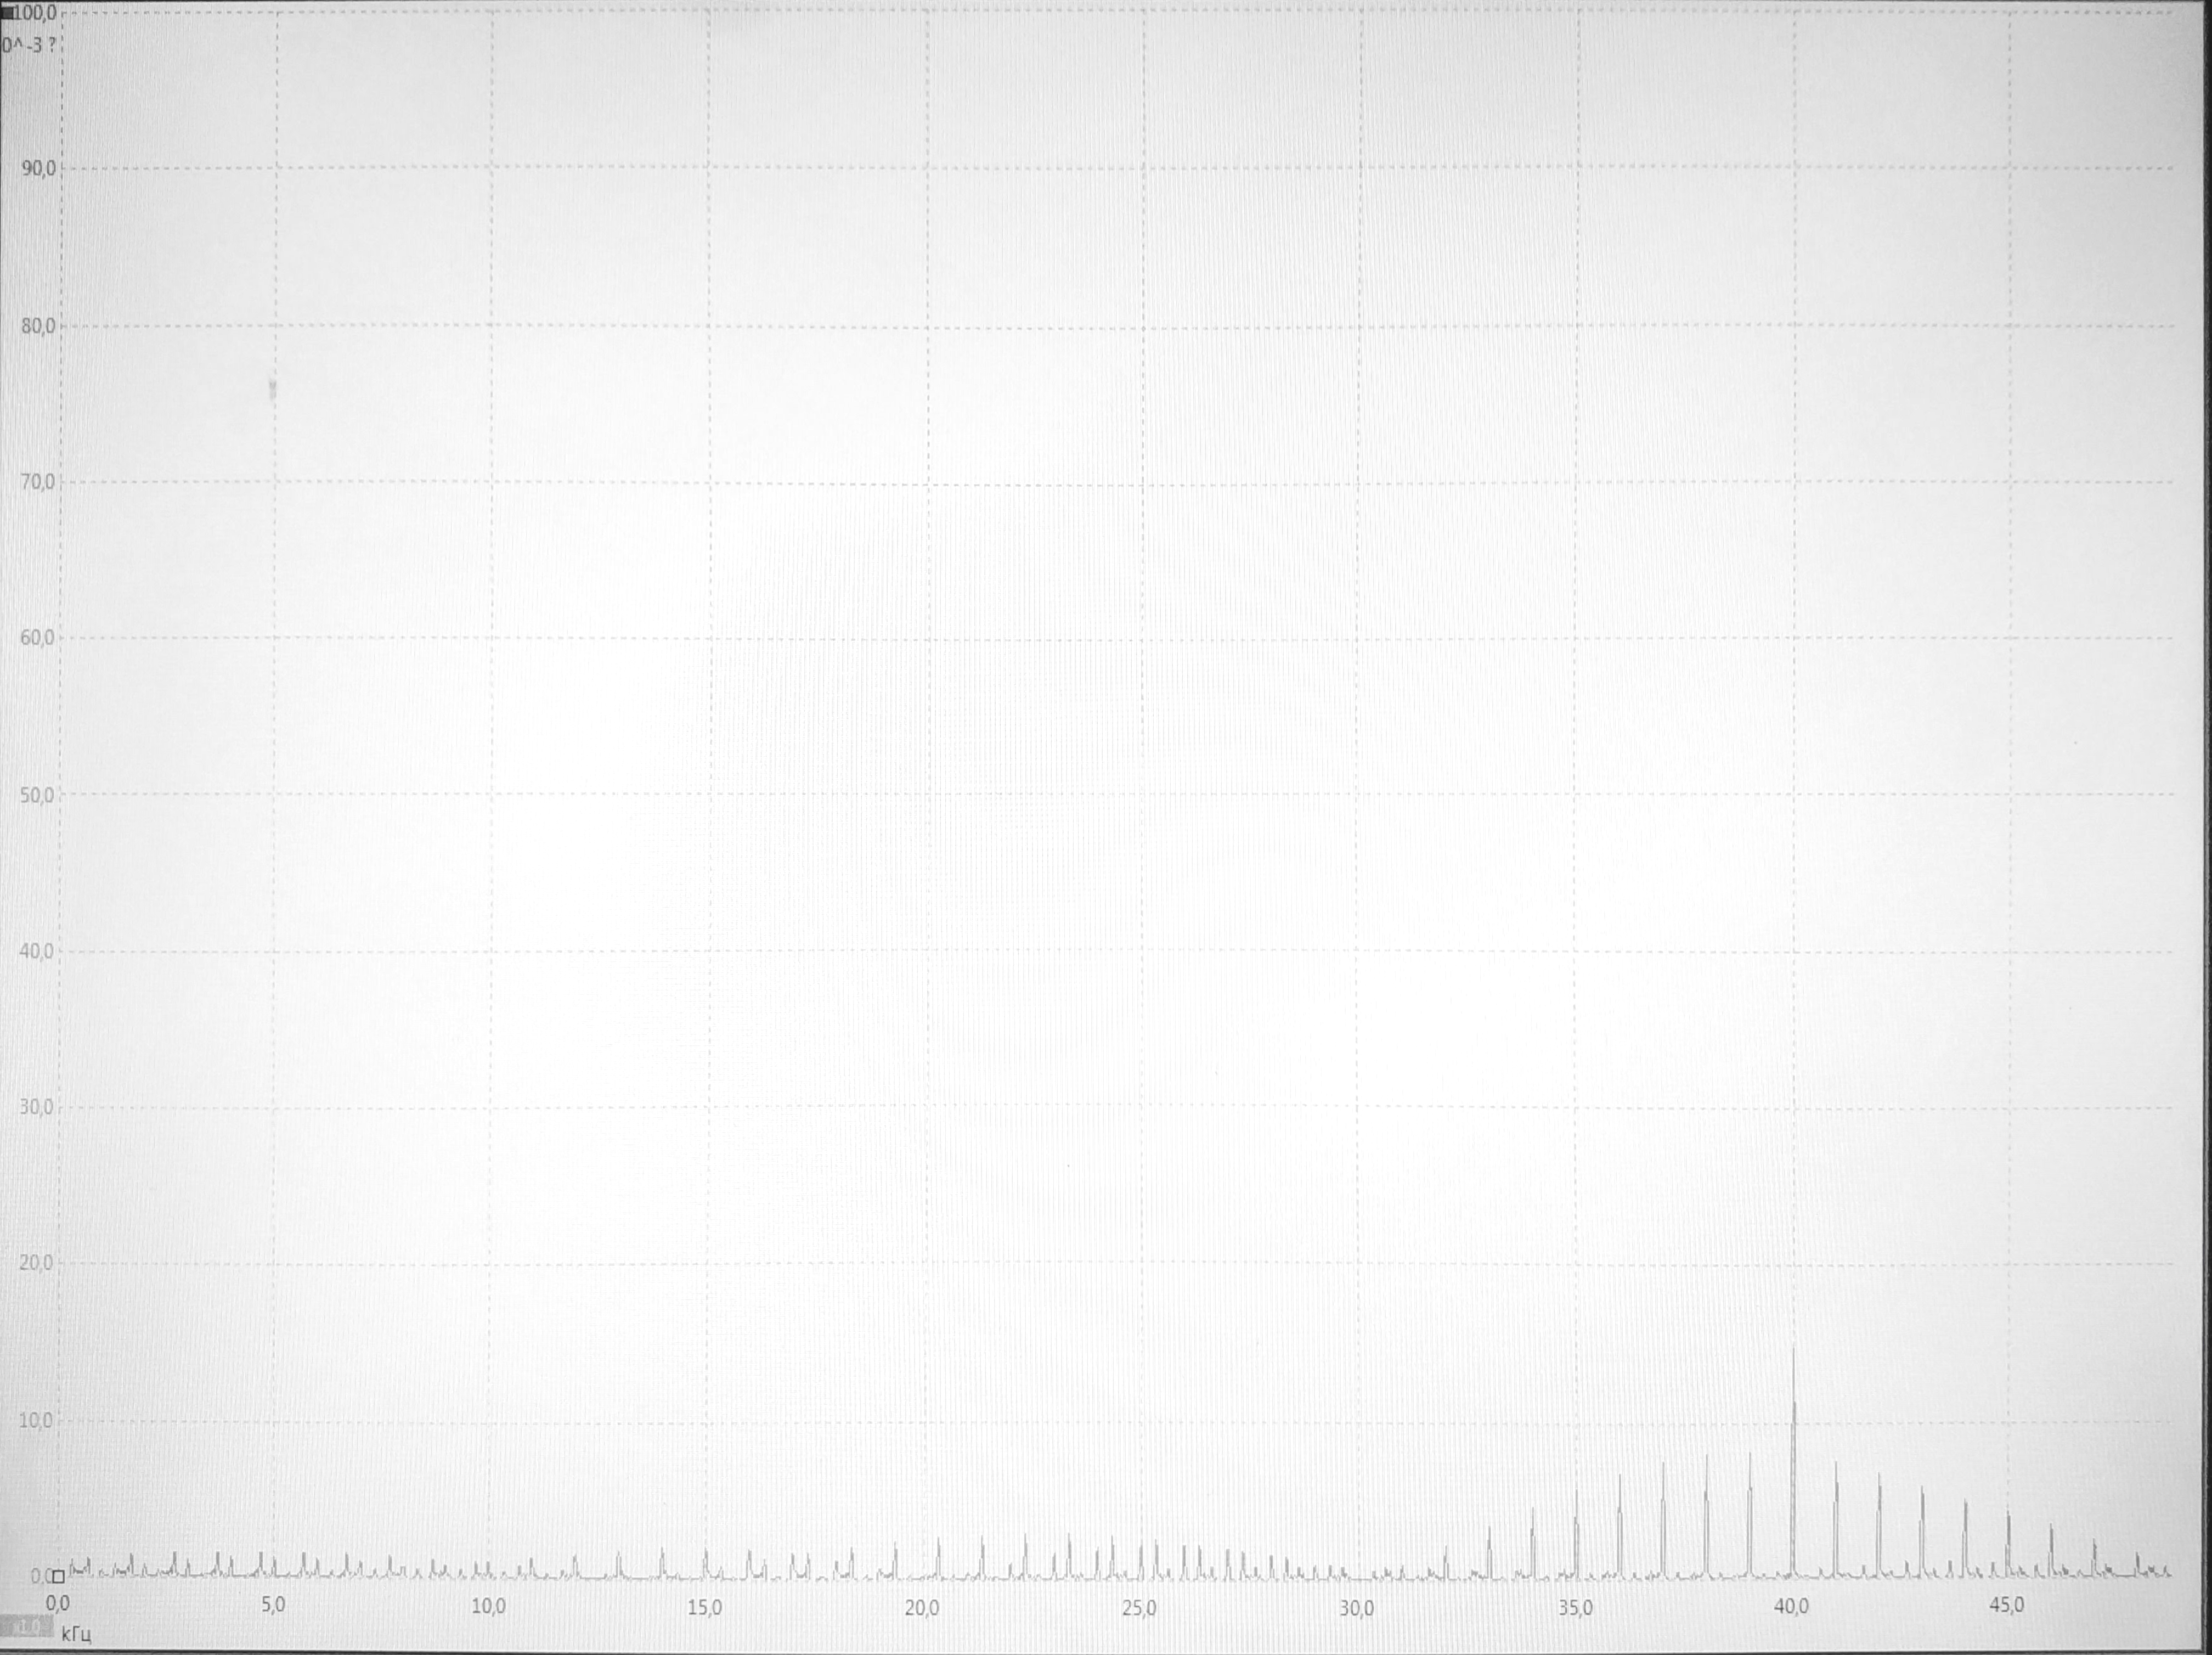
\includegraphics[width=0.85\linewidth]{img/13.jpg}

            При $\upsilon_0 = 40 \si{\kilo\hertz}$.
        \end{center}
        
        \newpage
        Определим зависимость расстояния $\delta v$ между соседними спектральными компонентами для разных частот повторения импульсов $f_{\text{повт}}$:
        
        \begin{center}
            \begin{tabular}{|c|l|l|l|l|l|}
                \hline
                N & 1&2&3&4&5  \\ \hline
                $\delta v, \si{\kilo\hertz}$ & 0.5 & 1& 2&4&5\\ \hline
                $f, \si{\kilo\hertz}$& 0.5 & 1&2&4&5 \\ \hline
            \end{tabular}
        \end{center}
        
        Построим график.
    
        \begin{center}
            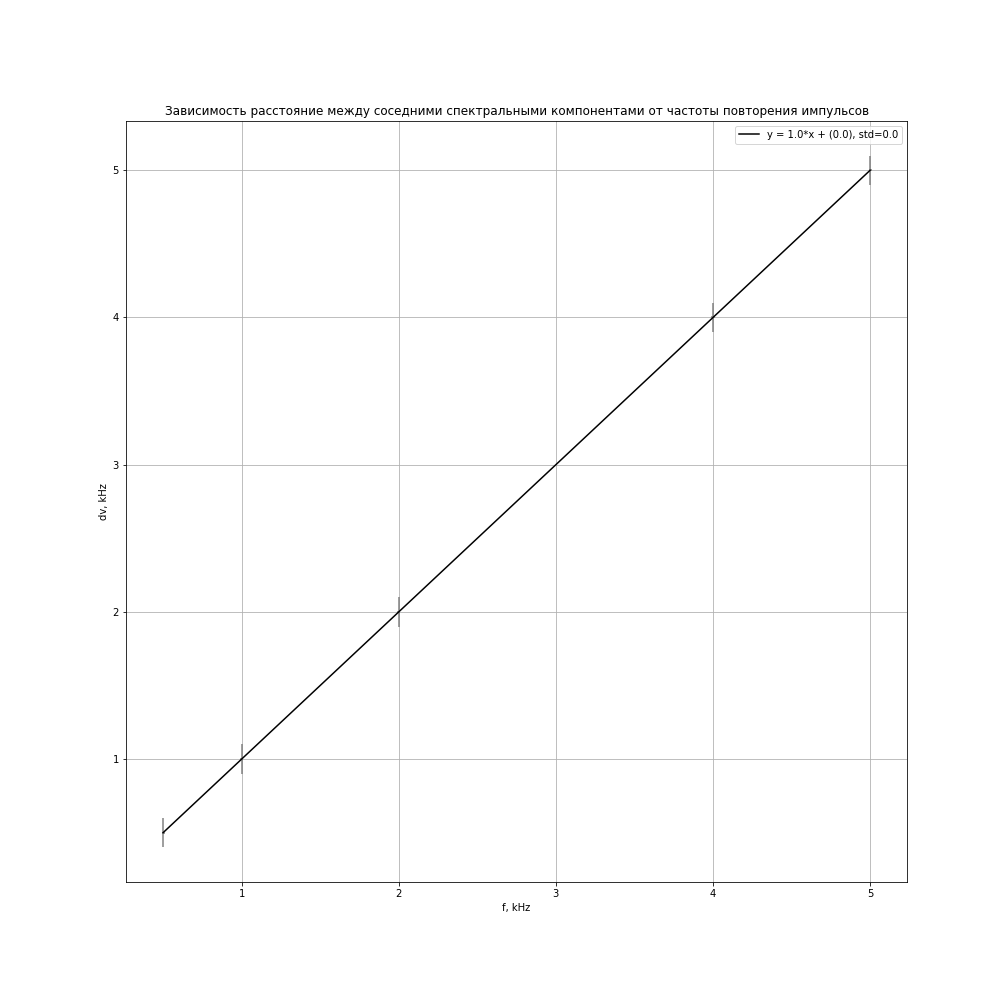
\includegraphics[width=\linewidth]{img/4.png}
        \end{center}
       
        \newpage
        Сравним спектры различных прямоугольных импульсов при $f_{\text{повт}} = 1000\si{\hertz}$ и цугов при $\tau = 100 \si{\micro\second}$:
        
        \begin{center}
            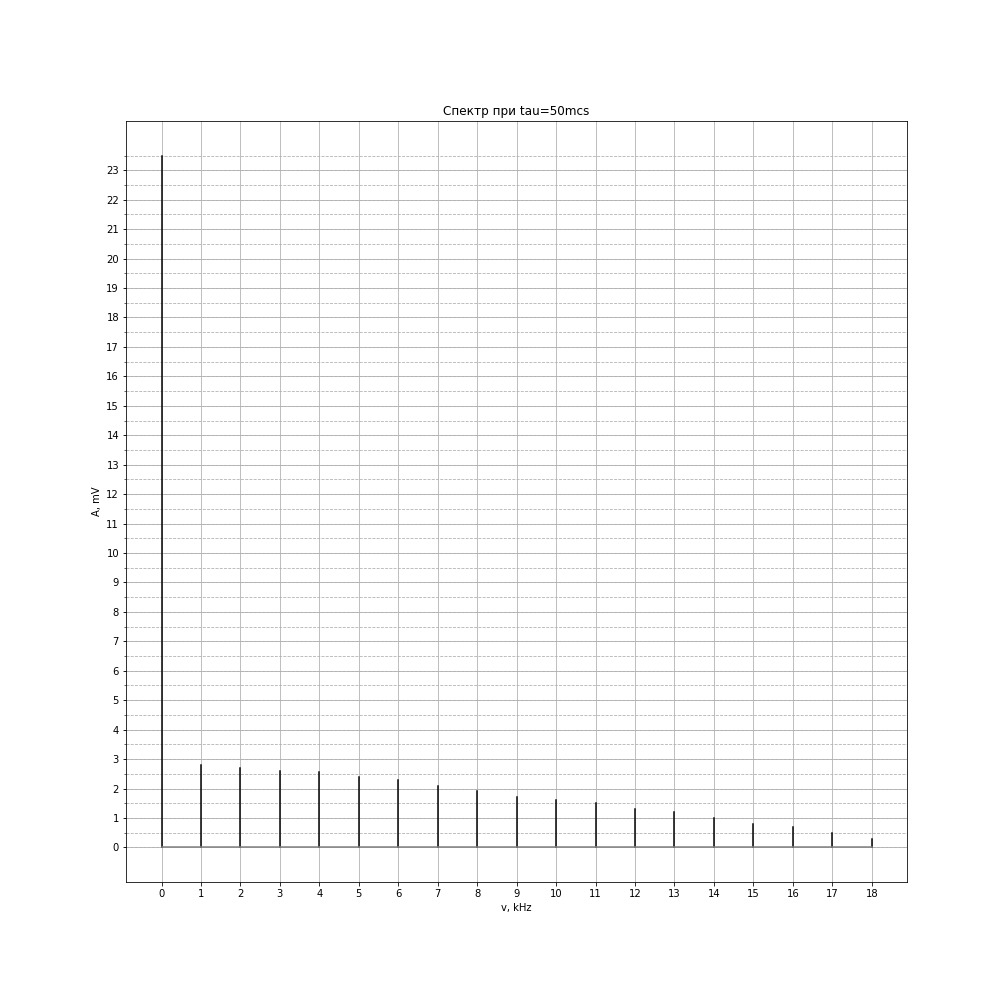
\includegraphics[width=0.65\linewidth]{img/2.png}
        
            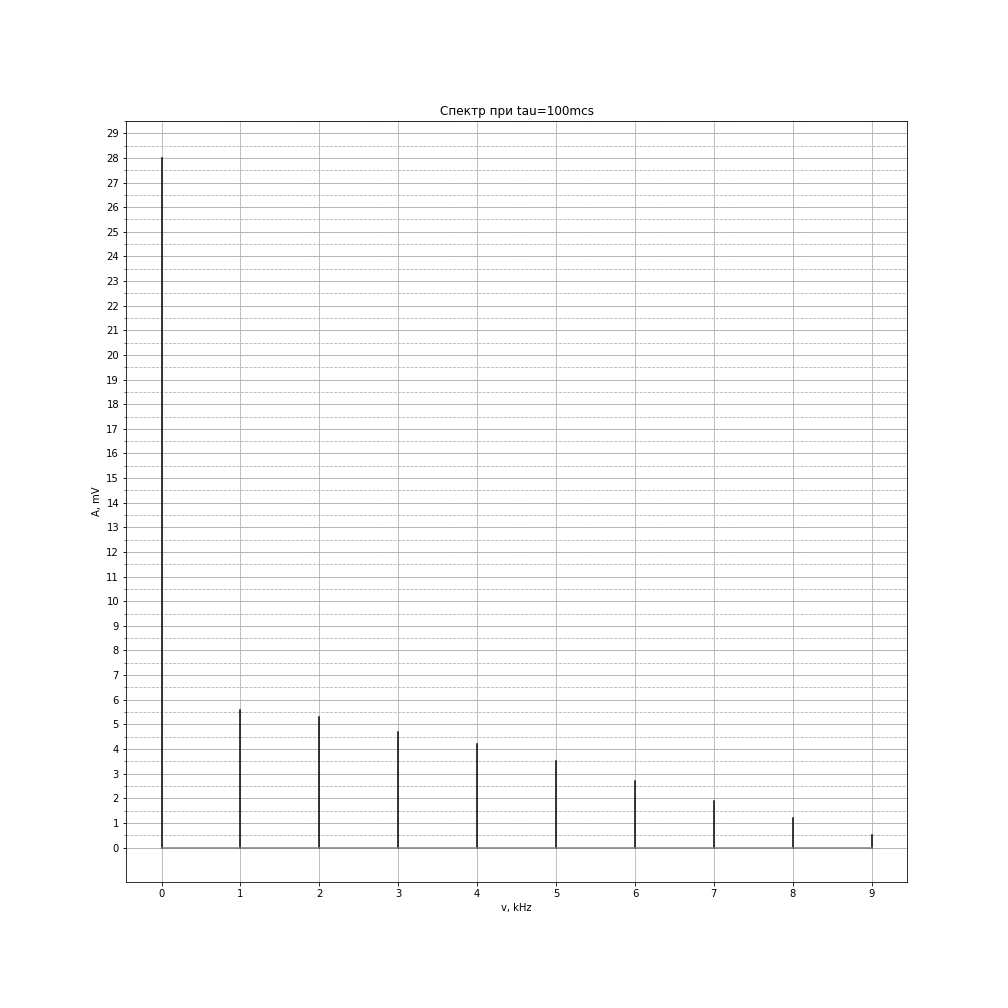
\includegraphics[width=0.65\linewidth]{img/3.png}
            
            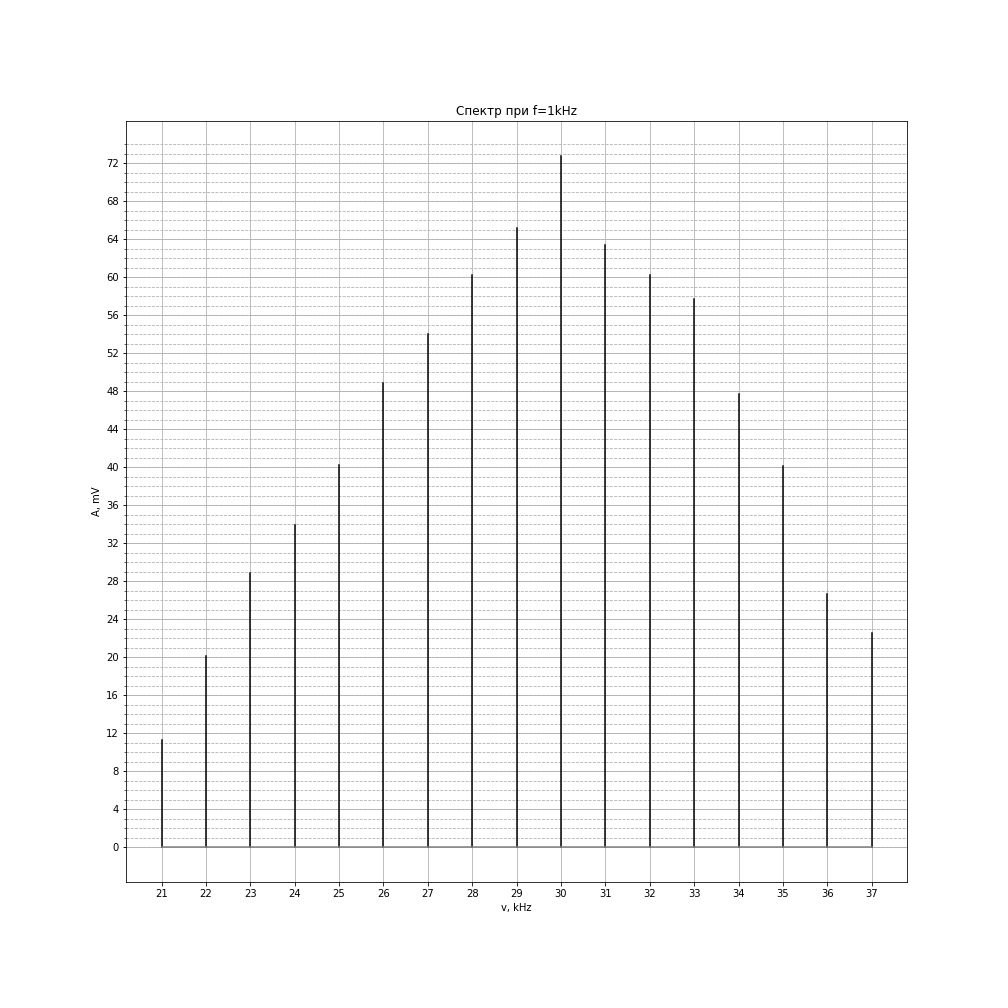
\includegraphics[width=0.65\linewidth]{img/5.png}
            
            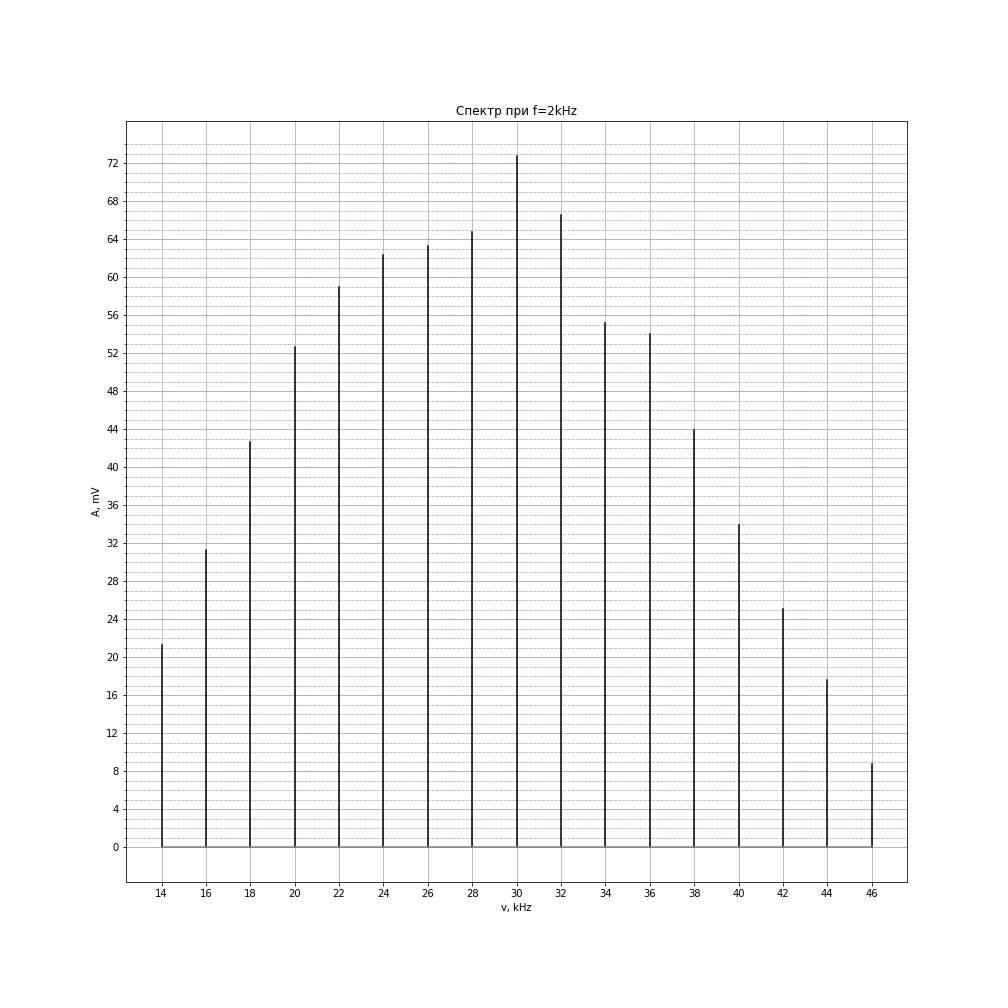
\includegraphics[width=0.65\linewidth]{img/6.png}   
        \end{center}

        
        \subsection{Исследуем спектры гармонических сигналов, модулированных по амплитуде.}
        \begin{center}
            \begin{tabular}{|c|l|l|l|l|l|l|l|l|}
                \hline
                {} &     $A \si{\volt}$ &  $A_{cent} \si{\volt}$ &  $A_{max} \si{\volt}$ &   $A_{min} \si{\volt}$ &  левый $A_{side} \si{\volt}$ &  правый $A_{side} \si{\volt}$ &   $mean A_{side} \si{\volt}$ &         m \\
                \hline
                0 &  0.20 &  0.6478 &  1.146 &  0.9200 &   0.0339 &   0.0339 &  0.03390 &  0.109390 \\
                1 &  0.65 &  0.6496 &  1.343 &  0.7036 &   0.1054 &   0.1016 &  0.10350 &  0.312421 \\
                2 &  1.10 &  0.6509 &  1.560 &  0.4969 &   0.1801 &   0.1719 &  0.17600 &  0.516846 \\
                3 &  1.55 &  0.6478 &  1.796 &  0.2214 &   0.2428 &   0.2428 &  0.24280 &  0.780510 \\
                4 &  2.00 &  0.6422 &  2.000 &  0.0000 &   0.3309 &   0.3090 &  0.31995 &  1.000000 \\
                \hline
            \end{tabular}    
        \end{center}
        
        Построим график отношения $A_{side}/A_{cent}$ в зависимости от $m$:
        
        \begin{center}
            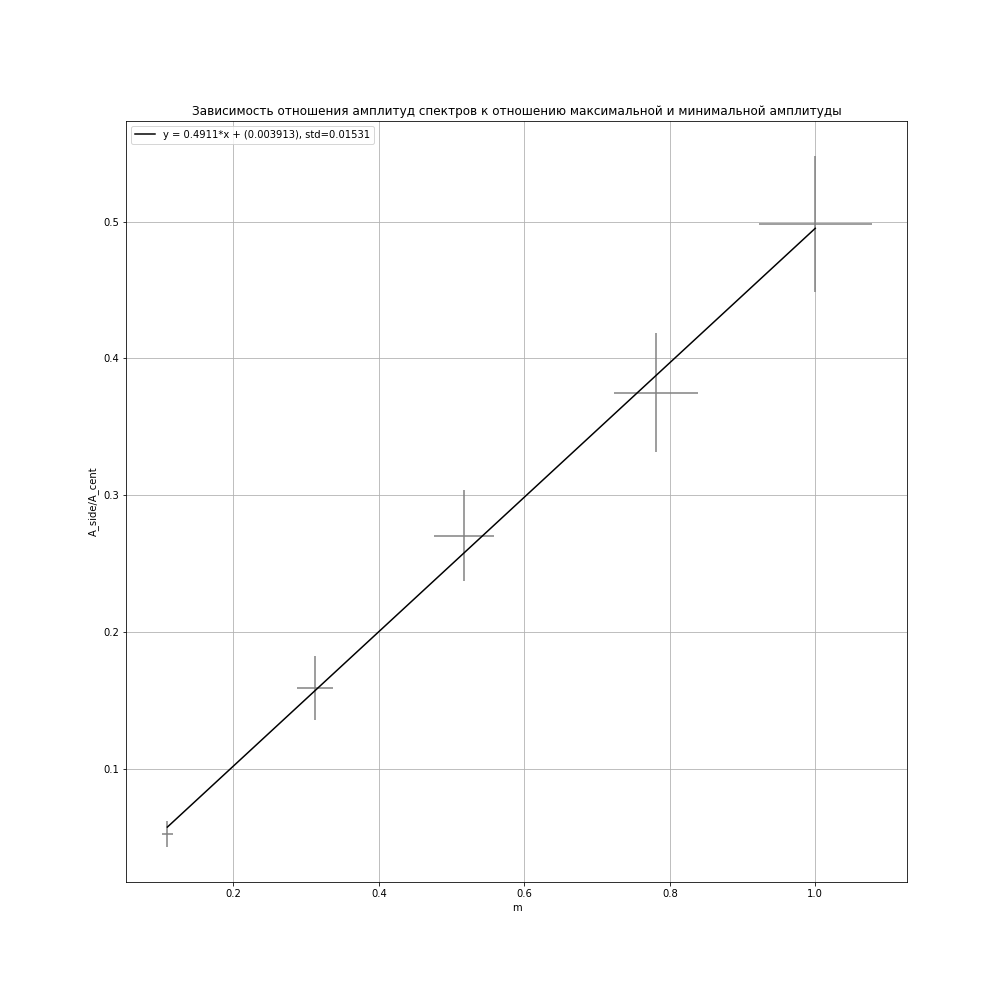
\includegraphics[width=\linewidth]{img/7.png}    
        \end{center}
        
\section{Вывод.}
    В работе был проведен спектральный анализ электрических спектров, представляющих из себя последовательность прямоугольных импульсов, последовательность цугов, амплитудно-модулированных гармонических колебаний.
    
    Проверено выполнение соотношений неопределнностей для первых двух видов спектра.
\end{document}
